% Compile with XeLaTeX.
\documentclass{article}
\usepackage[UTF8,scheme=plain,fontset=fandol]{ctex}
\usepackage{xcolor}
\usepackage{titleps}
\usepackage[letterpaper, margin=0.95in]{geometry}
\usepackage{url}
\usepackage{amsmath}
\usepackage{amssymb}
\usepackage{wrapfig}
\usepackage{float}
\usepackage{mathtools}
\usepackage{enumitem}
\usepackage{tabu}
\usepackage{parskip}
\usepackage{natbib}
\usepackage{listings}
\usepackage{forest}
\usepackage{hyperref}
\usepackage[color=red]{todonotes}
\usepackage{forest}
\definecolor{light-yellow}{HTML}{FFE5CC}

\usepackage{cleveref}
\usepackage{graphicx}

\newpagestyle{ruled}
{\sethead{RL2026fall / 95065}{增强学习}{Fall 2026}\headrule
  \setfoot{}{}{}}
\pagestyle{ruled}

\renewcommand\makeheadrule{\color{black}\rule[-.75\baselineskip]{\linewidth}{0.4pt}}
\renewcommand*\footnoterule{}

\begin{document}
\lstset{basicstyle = \ttfamily,columns=fullflexible,
backgroundcolor = \color{light-yellow}
}

\begin{centering}
    {\Large [SOLUTION TEMPLATE] Assignment 1: Imitation Learning} \\
    \vspace{.25cm}
    \textbf{提交截止日期见课程站点} \\
    \vspace{.15cm}
    提交入口：\url{https://oc.sjtu.edu.cn/courses/95065} \\
    \vspace{.15cm}
    姓名：潘昊辰 \quad 学号：523120910233 \\
\end{centering}

\vspace{0.5cm}

\section{Introduction}

The goal of this assignment is to experiment with imitation learning, including direct \textbf{behavior cloning} and the \textbf{DAgger} algorithm.
The methods we learn about in this assignment will lay the groundwork for subsequent assignments where we explore more advanced reinforcement learning techniques.

In \textbf{Behavior Cloning (BC)}, we treat imitation learning as a supervised learning problem: given a dataset of expert demonstrations $\mathcal{D} = \{(s_i, a_i)\}$, we train a policy $\pi_\theta$ to minimize:
\[
\min_\theta \; \mathbb{E}_{(s,a)\sim\mathcal{D}} \left[\| \pi_\theta(s) - a \|^2 \right]
\]
(or the equivalent negative log-likelihood loss for a stochastic policy).

In \textbf{DAgger (Dataset Aggregation)}, we iteratively:
\begin{enumerate}
    \item Use the current policy $\pi_\theta$ to roll out trajectories in the environment;
    \item Query the expert policy to relabel the visited states with expert actions;
    \item Aggregate the new data into the training set and retrain $\pi_\theta$.
\end{enumerate}
This procedure addresses the \emph{distribution shift} problem inherent in behavior cloning, where the learner encounters states outside the expert's demonstration distribution.

\subsection{Code}

Files to edit (fill in \texttt{TODO} sections):
\begin{itemize}
    \item \verb|sjtuRL2026/policies/MLP_policy.py| --- MLP policy: \texttt{forward()} and \texttt{update()}.
    \item \verb|sjtuRL2026/infrastructure/utils.py| --- \texttt{sample\_trajectory()}: collect a single rollout.
    \item \verb|sjtuRL2026/scripts/run_hw1.py| --- Training loop:
    \begin{itemize}
        \item DAgger data collection: \verb|utils.sample_trajectories()|
        \item Expert relabeling of collected observations
        \item Sampling from replay buffer for gradient updates
    \end{itemize}
\end{itemize}

\subsection{Running the Code}

Behavior Cloning example (Ant):
\begin{lstlisting}
python sjtuRL2026/scripts/run_hw1.py \
  --expert_policy_file sjtuRL2026/policies/experts/Ant.pkl \
  --env_name Ant-v4 --exp_name bc_ant --n_iter 1 \
  --expert_data sjtuRL2026/expert_data/expert_data_Ant-v4.pkl \
  --video_log_freq -1
\end{lstlisting}

DAgger example (Ant, 10 iterations):
\begin{lstlisting}
python sjtuRL2026/scripts/run_hw1.py \
  --expert_policy_file sjtuRL2026/policies/experts/Ant.pkl \
  --env_name Ant-v4 --exp_name dagger_ant --n_iter 10 \
  --do_dagger \
  --expert_data sjtuRL2026/expert_data/expert_data_Ant-v4.pkl \
  --video_log_freq -1
\end{lstlisting}

Available environments: \verb|Ant-v4|, \verb|Walker2d-v4|, \verb|HalfCheetah-v4|, \verb|Hopper-v4|.

Tip: use \verb|--video_log_freq -1| during debugging to disable video logging.

%%%%%%%%%%%%%%%%%%%%%%%%%%%%%%%%%%%%%%%%%%%%%
\newpage
\section{Section 1: Behavior Cloning}
%%%%%%%%%%%%%%%%%%%%%%%%%%%%%%%%%%%%%%%%%%%%%

\subsection{BC Results Table}
\begin{itemize}
    \item Run BC (\verb|n_iter=1|) on at least one environment.
    \item Report the mean and standard deviation of evaluation returns (\verb|Eval_AverageReturn|, \verb|Eval_StdReturn|).
    \item Include: environment name, \verb|ep_len|, \verb|eval_batch_size|, network architecture (layers $\times$ hidden units), training steps, expert data size.
    \item Note: ensure \verb|eval_batch_size| $>$ \verb|ep_len| so that multiple trajectories are evaluated, making mean/std meaningful.
\end{itemize}

\textbf{Solution:}

\begin{table}[H]
\centering
\begin{tabular}{|l|c|c|c|}
\hline
\textbf{环境} & \textbf{评估平均回报} & \textbf{评估回报标准差} & \textbf{专家平均回报} \\
\hline
Ant-v4 & 976.30 & 195.69 & 4681.89 \\
HalfCheetah-v4 & 3236.47 & 93.13 & 4034.80 \\
\hline
\end{tabular}
\caption{BC 在两个环境上的实验结果。网络用了 2 层隐藏层 $\times$ 64 单元，激活函数 Tanh，学习率 5e-3，训练了 1000 个梯度步，batch size 100。}
\end{table}

实验设置：\verb|ep_len|=1000，\verb|eval_batch_size|=5000（每次评估采 5 条轨迹，所以报告的标准差是有意义的），\verb|batch_size|=1000，每个环境用的专家数据是 2 条轨迹（共 2000 个转移），\verb|seed|=1。

BC 在两个环境上的表现都没追上专家。Ant 上大概只有专家回报的 21\%，HalfCheetah 好一些，约在 80\% 左右。差距主要是\emph{分布漂移}（distribution shift）造成的：测试时策略遇到的是专家演示里没出现过的新状态，误差会沿着整条轨迹一步步放大。Ant 上这个问题更严重，因为它的动力学更复杂，智能体很容易滑到没法恢复的局面。

\subsection{Hyperparameter Experiment}
\begin{itemize}
    \item Choose at least one hyperparameter that significantly affects BC performance. Possible choices include:
    \begin{itemize}
        \item Number of training gradient steps (\verb|num_agent_train_steps_per_iter|)
        \item Amount of expert data (subset vs.\ full)
        \item Network architecture (number of layers, hidden layer width)
    \end{itemize}
    \item Keep all other settings fixed and vary only the chosen hyperparameter on the \textbf{same} environment.
    \item Plot ``BC performance (\verb|Eval_AverageReturn|) vs.\ chosen hyperparameter''.
    \item In the caption, describe:
    \begin{itemize}
        \item Which hyperparameter was varied and its range
        \item Why this hyperparameter affects BC performance
        \item Other key settings (environment, \verb|ep_len|, \verb|eval_batch_size|, etc.)
    \end{itemize}
\end{itemize}

\textbf{Solution:}

\begin{figure}[H]
\centering
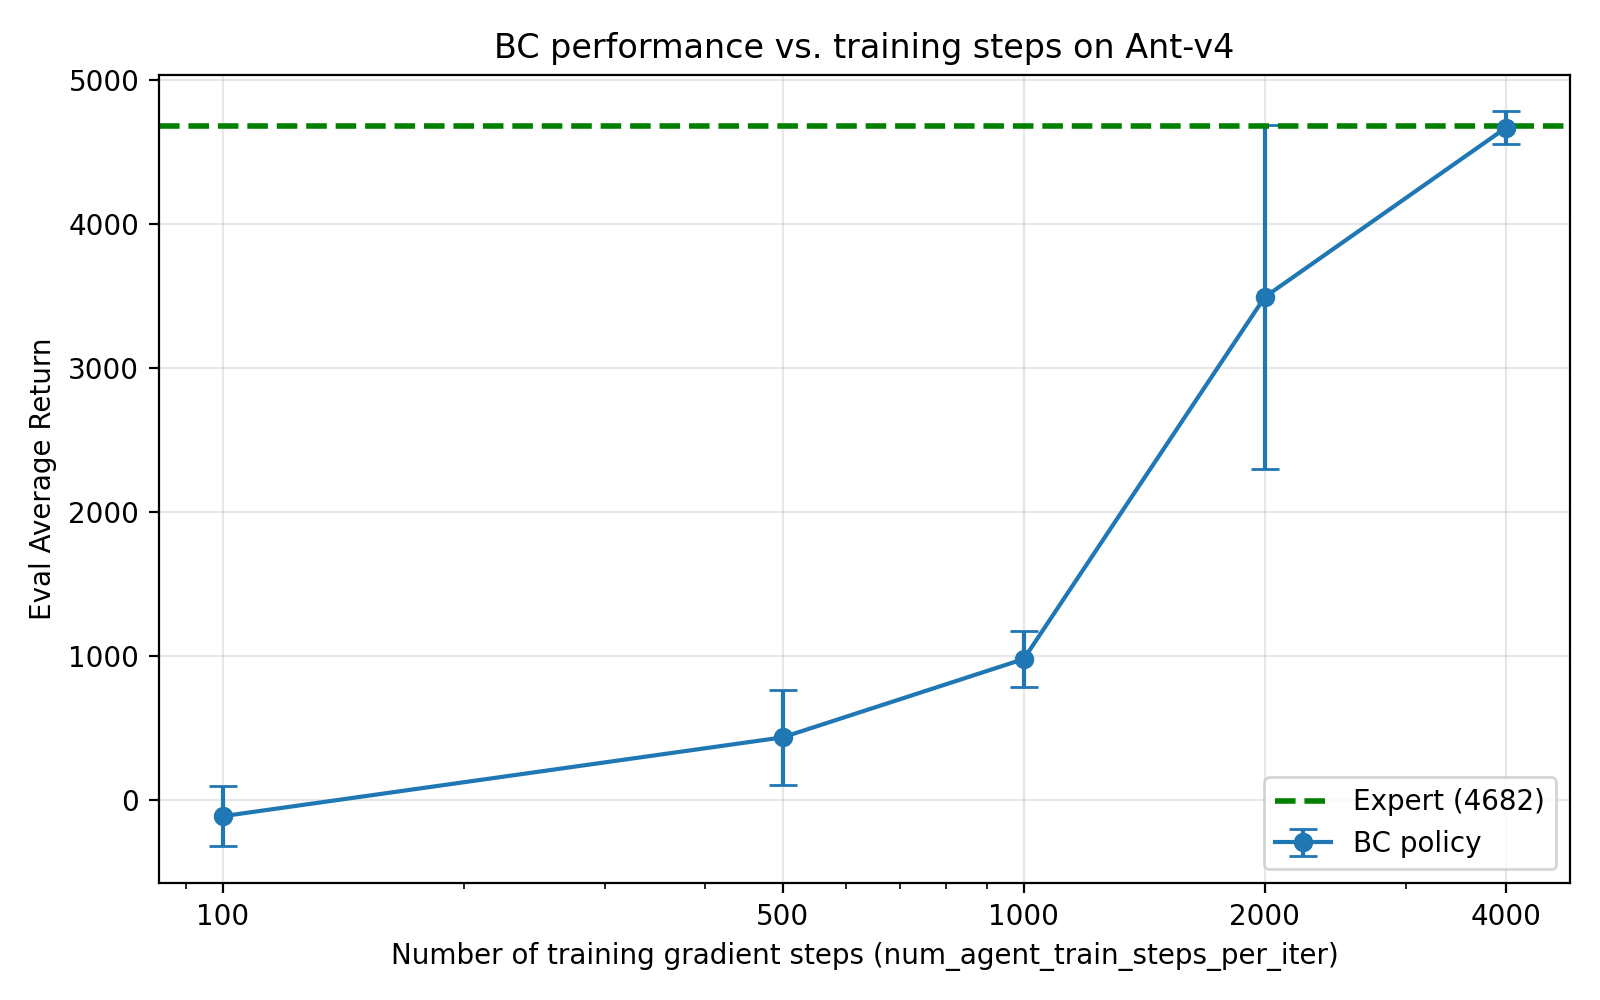
\includegraphics[width=0.75\textwidth]{bc_hyperparam.png}
\caption{BC 在 Ant-v4 上随训练梯度步数的变化。步数取了 $\{100, 500, 1000, 2000, 4000\}$ 这几个值，其他设置都没动：\texttt{ep\_len}=1000，\texttt{eval\_batch\_size}=5000（测了 5 条轨迹），网络是 2$\times$64 的 Tanh，学习率 5e-3，训练 batch size 100，专家数据用了 2 条轨迹（2000 个转移）。步数越多，策略对专家数据拟合得越好，回报也跟着往上走；到 4000 步的时候已经离专家很近了（4667.79 对 4681.89）。误差棒对应的是 5 条评估轨迹的 Eval\_StdReturn。}
\end{figure}

下面几组命令每次只改 \verb|--num_agent_train_steps_per_iter| 的值，分别跑了 100、500、1000、2000、4000 这几个步数：
\begin{lstlisting}
python sjtuRL2026/scripts/run_hw1.py \
  --expert_policy_file sjtuRL2026/policies/experts/Ant.pkl \
  --env_name Ant-v4 --exp_name bc_ant_steps<N> --n_iter 1 \
  --expert_data sjtuRL2026/expert_data/expert_data_Ant-v4.pkl \
  --video_log_freq -1 --eval_batch_size 5000 \
  --num_agent_train_steps_per_iter <N>
\end{lstlisting}

%%%%%%%%%%%%%%%%%%%%%%%%%%%%%%%%%%%%%%%%%%%%%
\newpage
\section{Section 2: DAgger}
%%%%%%%%%%%%%%%%%%%%%%%%%%%%%%%%%%%%%%%%%%%%%

\subsection{DAgger Learning Curve}
\begin{itemize}
    \item Run DAgger (\verb|--do_dagger --n_iter 10| or more) on at least one environment (preferably the same as your BC experiment).
    \item Plot ``DAgger iteration vs.\ \verb|Eval_AverageReturn|'' with error bars (\verb|Eval_StdReturn|):
    \begin{itemize}
        \item $x$-axis: DAgger iteration number (0 = pure BC warmstart, 1, 2, \dots)
        \item $y$-axis: \verb|Eval_AverageReturn|
    \end{itemize}
    \item On the same plot, include horizontal baselines:
    \begin{itemize}
        \item \textbf{Expert policy} performance (dashed green line)
        \item \textbf{BC-only} performance (dashed red line, i.e., iteration 0)
    \end{itemize}
    \item In the caption, state: environment, network architecture, \verb|ep_len|, \verb|eval_batch_size|, expert data size, and other relevant hyperparameters.
\end{itemize}

\textbf{Solution:}

\begin{figure}[H]
\centering
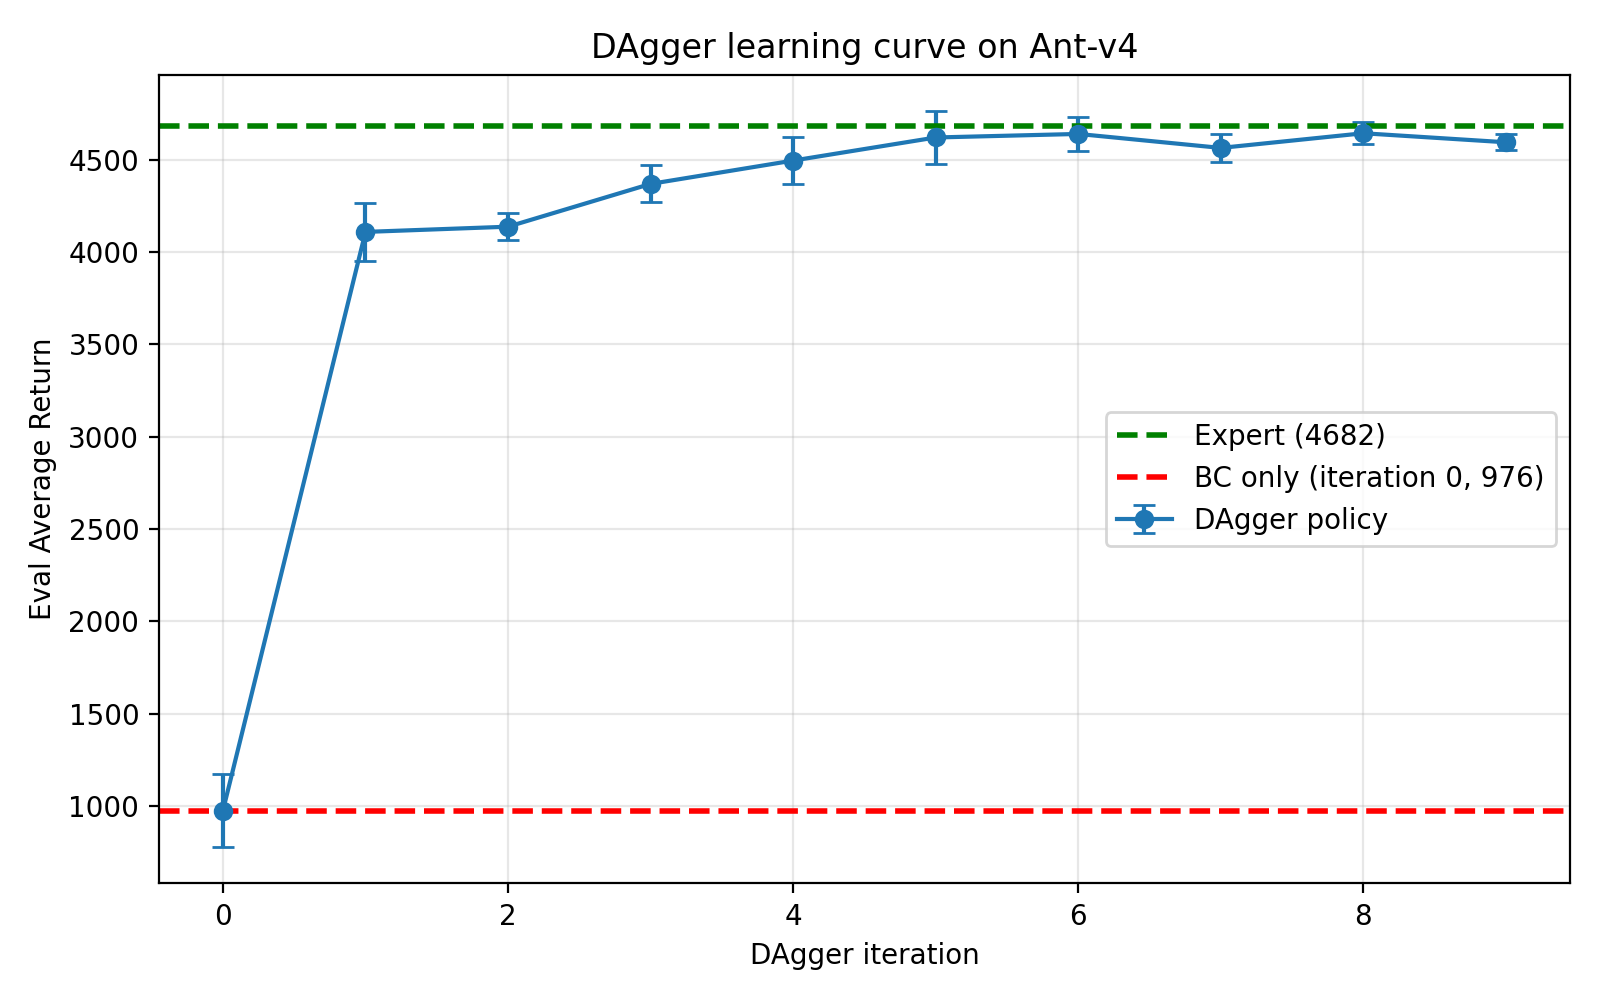
\includegraphics[width=0.75\textwidth]{dagger_curve.png}
\caption{DAgger 在 Ant-v4 上的学习曲线。横轴是迭代轮数，第 0 轮是纯 BC 预热（只用专家数据），之后 1\textasciitilde 9 轮是 DAgger 迭代。纵轴是 Eval\_AverageReturn，误差棒来自 Eval\_StdReturn。绿色虚线是专家策略的平均回报（4681.89），红色虚线是 BC-only 基线（976.30）。实验设置和前面一致：\texttt{ep\_len}=1000，\texttt{eval\_batch\_size}=5000（5 条轨迹），网络 2$\times$64（Tanh），学习率 5e-3，训练 batch size 100，专家数据 2 条轨迹（2000 个转移），每轮 \texttt{num\_agent\_train\_steps\_per\_iter}=1000。}
\end{figure}

完整的命令如下：
\begin{lstlisting}
python sjtuRL2026/scripts/run_hw1.py \
  --expert_policy_file sjtuRL2026/policies/experts/Ant.pkl \
  --env_name Ant-v4 --exp_name dagger_ant_final --n_iter 10 --do_dagger \
  --expert_data sjtuRL2026/expert_data/expert_data_Ant-v4.pkl \
  --video_log_freq -1 --eval_batch_size 5000
\end{lstlisting}

\subsection{BC vs.\ DAgger Comparison}
\begin{itemize}
    \item Briefly discuss:
    \begin{itemize}
        \item How does DAgger compare to BC-only?
        \item Does DAgger approach expert-level performance? After how many iterations?
        \item What is the effect of distribution shift, and how does DAgger address it?
    \end{itemize}
\end{itemize}

\textbf{Solution:}

\textbf{DAgger 与 BC-only 的对比。} 只跑 BC 的话，Ant 上的回报只有 976.30，大概是专家的 21\%。DAgger 的效果明显好很多：第一轮迭代后就冲到了 4108.44，从第 5 轮开始就基本稳定在 4600\textasciitilde 4670 的区间里，最后算下来差不多是 BC-only 的 4.7 倍。

\textbf{是否达到专家水平。} DAgger 在 5 轮之内就已经接近专家水平了，第 5 轮 4619.60，第 9 轮 4593.69，和专家回报 4681.89 的差距基本在 2\% 左右。进步最明显的是第 0 轮到第 1 轮之间，一下子从 976.30 跳到了 4108.44，后面因为策略已经进入了高回报的状态区域，提升就变得比较平缓了。

\textbf{分布漂移的影响与 DAgger 的解决方式。} BC 出问题主要是因为分布漂移。策略在测试时碰到的是专家演示里没出现过的状态，在 Ant 上这些没见过的情况会让误差越攒越多，智能体很容易失控到没法恢复的局面，所以回报只有专家的 21\%。DAgger 的做法其实挺直观的，分三步走：（1）先用当前策略在环境里跑，看看它到底会进哪些状态；（2）让专家给这些状态重新标上正确的动作；（3）把新数据加进训练集。这样训练分布就能跟上测试时真正遇到的情况，策略就算碰到专家以前没展示过的状态也能学怎么应对。

%%%%%%%%%%%%%%%%%%%%%%%%%%%%%%%%%%%%%%%%%%%%%
\newpage
\section{提交说明：仅提交 PDF 报告}

完成实验后，在 \texttt{hw1\_template.tex} 中填写答案、实验设置、结果表格、曲线和分析，并在报告中注明姓名与学号。所有必需的实验结果均应包含在报告内。

使用 XeLaTeX 编译报告。在模板所在目录运行：
\begin{lstlisting}
xelatex hw1_template.tex
xelatex hw1_template.tex
\end{lstlisting}
生成文件为 \texttt{hw1\_template.pdf}。

如使用 Overleaf，请选择 XeLaTeX 编译器，以 \texttt{hw1\_template.tex} 为主文档，编译后下载 PDF。

\textbf{最终只需上传填写完整的 PDF 报告，无需上传代码、实验日志、视频、TeX 源文件或 ZIP 压缩包。} 代码与日志请自行保留，供生成图表与核查结果使用。提交前请打开 PDF，检查图表、公式及答案是否显示完整。

提交入口：\url{https://oc.sjtu.edu.cn/courses/95065}。截止日期以课程平台通知为准。

\newpage
\section{Visualization (Optional)}

Use TensorBoard to inspect your training logs:

\begin{lstlisting}
tensorboard --logdir data
\end{lstlisting}

You will see scalar summaries (e.g., \verb|Eval_AverageReturn|, \verb|Training Loss|) as well as videos of your trained policies (in the ``Images'' tab, if video logging was enabled).

To compare specific runs:
\begin{lstlisting}
tensorboard --logdir data/run1,data/run2,data/run3
\end{lstlisting}

You can also use the provided \verb|scripts/run_hw1.ipynb| notebook to extract data from TensorBoard event files and produce publication-quality plots.

\newpage
\section{Survey}
\label{sec:survey}
Please estimate, in minutes, for each section, how much time you spent (a) writing code and (b) waiting for the results. This will help us calibrate the difficulty for future homeworks.
\begin{itemize}
    \item \textbf{Behavior Cloning (coding):} 50 分钟
    \item \textbf{Behavior Cloning (experiments):} 100 分钟
    \item \textbf{DAgger (coding):} 25 分钟
    \item \textbf{DAgger (experiments):} 60 分钟
\end{itemize}

\end{document}
